\subsection*{Paikkajärjestelmät}

Merkitsemme lukuja yleensä \termi{kymmenjärjestelmä}{kymmenjärjestelmässä} eli \termi{lukujärjestelmä}{lukujärjestelmässä}, jossa on kymmenen \termi{numeromerkki}{numeromerkkiä}: 0, 1, 2, 3, 4, 5, 6, 7, 8 ja 9. (Käyttämämme numeromerkit ovat nimeltään hindu-arabialaiset numerot.) Kymmenjärjestelmää kutsutaan myös \termi{desimaalijärjestelmä}{desimaalijärjestelmäksi}. Tunnetaan kulttuureja, joissa on käytetty pääasiallisesti jotakin muuta lukujärjestelmää.

Kymmenjärjestelmä on \termi{paikkajärjestelmä}{paikkajärjestelmä}, eli merkin paikka määrittää sen merkityksen.

\begin{esimerkki}
Numeron 8 merkitys riippuu sen paikasta. Luvussa $80$ merkin 8 merkitys on $8 \cdot 10^1$, mutta luvussa $820$ sen merkitys on $8 \cdot 10^2$.
\end{esimerkki}
%viittaus desimaalilukukappaleeseen?
\begin{esimerkki}
Esitä luku $2\,080,7$ kymmenen potenssien summana.
	\begin{esimratk}
	$2\,090,7=2\cdot10^3+0\cdot10^2+0\cdot10^1+0\cdot10^0+7\cdot10^{-1}$
	\end{esimratk}
\end{esimerkki}

Nykyään yleisimmät desimaalijärjestelmästä poikkeavat lukujärjestelmät ovat \termi{binäärijärjestelmä}{binääri}-, \termi{oktaalijärjestelmä}{oktaali}- ja \termi{heksadesimaalijärjestelmä}{heksadesimaalijärjestelmät}, joissa on vastaavasti $2$, $8$ ja $16$ numeromerkkiä. Tietokoneet käsittelevät lukuja sisäisesti binäärijärjestelmässä, kun taas oktaali- ja heksadesimaalijärjestelmät ovat muutoin käteviä tietojenkäsittelytieteessä.

Yleisesti pätee, että kun käytettävissä olevien merkkien määrää lisää, suuria lukuja voi kirjoittaa lyhyempään muotoon. Näin ollen sama luku esitettynä kolmekantaisessa lukujärejstelmässä voi olla paljon pidempi kuin kymmenkantaisessa esitettynä. Tilanne on verrattavissa vaikkapa kiinan kieleen, jossa on käytössä tuhansia erilaisia kirjoitusmerkkejä. Merkeissä on paljon muistettavaa, mutta toisaalta kokonaisen lauseen voi kirjoittaa vain parilla kirjoitusmerkillä.

Binäärijärjestelmässä luvun muodostavia numeromerkkejä kutsutaan \termi{bitti}{biteiksi}. Bitti voi olla joko päällä (1) tai pois päältä (0), ja toteutus tietokoneessa vastaa esimerkiksi sitä, että johtimessa kulkee virta (1) tai ei (0). Kuusitoistajärjestelmässä tarvitaan numeroiden $0 \ldots \, 9$ lisäksi kuusi uutta numeromerkkiä. Tavaksi on vakiintunut käyttää kirjainmerkkejä $\mathrm{A, B, C, D, E, F}$. Ne vastaavat desimaalilukuja $10 \ldots \, 15$.

Useampaa järjestelmää käytettäessä, erityisesti muunnettaessa lukuja järjestelmästä toiseen, merkitään kantaluku luvun jälkeen alaindeksinä. Voimme esimerkiksi merkitä (desimaalijärjestelmän) lukua yhdeksäntoista $10011_2$, $23_8$, $19_{10}$ tai $13_{16}$. Huomaa, että binäärijärjestelmän luvuissa ei ole mielekästä käyttää tuhaterotinta, koska sana tuhat itsessään viittaa kymmenjärjestelmälle ominaiseen kolmanteen kymmenen potenssiin. Binääriluvuille ei ole vakiintunut vastaavia ilmaisuja kuten sata tai miljoona, vaan luvut luetaan numero kerrallaan.

\begin{esimerkki}
Luku $11001_2$ luetaan "yksi yksi nolla nolla yksi".
\end{esimerkki}

Luvut eri kannoissa voidaan muuttaa desimaaliluvuiksi esittämällä luku potenssien summina kymmenjärejstelmässä.

%alaviitemerkintä

\begin{esimerkki}
$10,01_2 = 1 \cdot 2^1 + 0 \cdot 2^0 + 0 \cdot 2^{-1} + 1 \cdot 2^{-2} = 2,25_{10}$
\end{esimerkki} %pitää kirjoittaa näitä muunnosesimerkkejä :/

%\begin{esimerkki}
%Millä kantaluvulla $n$ pätee yhtälö $10_n+10_n=$ ... (tulee potensisyhtälö,tuntematon kantaluku)
%\end{esimerkki}

Lukujärjestelmiä voidaan vaihtoehtoisesti merkitä kirjoittamalla niiden tunnus (Bin, Oct, Dec, Hex) luvun jälkeen. Klassinen vitsi ''Miksi tietojenkäsittelytieteilijä sekoittaa halloweenin ja joulun? Koska $31$ Oct $= 25$ Dec!'' perustuu siihen, että

\begin{align*}
	\text{halloween} \; = \; \text{31. lokakuuta} \; &= \; \text{31 Oct} \; = 31_8 = 3_{10} \cdot 8_{10} + 1_{10} \cdot 1_{10} \\
	= {25}_{10} &= \; \text{25 Dec} \; = \; \text{25. joulukuuta} \; = \; \text{joulupäivä.}
\end{align*} %välit, siistimistä?

\subsection*{Muut lukujärjestelmät}

Yleisesti tunnetaan myös joitakin lukujärjestelmiä, jotka eivät ole paikkajärjestelmiä.

\termi{tukkimiehen kirjanpito}{Tukkimiehen kirjanpidossa} toistetaan yhtä ainoaa merkkiä. Se on tavallaan 1-järjestelmä, mutta tällainen määrittely ei ole ongelmaton.

\begin{center}
	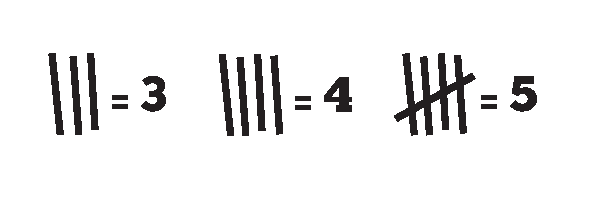
\includegraphics{pictures/Kuva1-1-tukkimiehenkirjanpito.pdf}
\end{center}

Hienostuneempi versio tukkimiehen kirjanpidosta ovat \termi{roomalaiset luvut}{roomalaiset luvut}, jotka nimensä mukaisesti olivat yleisin lukujärjestelmä antiikin Roomassa. Roomalaisia lukuja käytetään yhä nykyäänkin erityisesti järjestyksen merkitsemisessä. Roomalaisten lukujen numeromerkit ovat I, V, X, L, C, D ja M. Ne vastaavat desimaalijärjestelmän lukuja seuraavalla tavalla:

\begin{equation*}
	\textrm{I}=1\quad
	\textrm{V}=5\quad
	\textrm{X}=10\quad
	\textrm{L}=50\quad
	\textrm{C}=100\quad
	\textrm{D}=500\quad
	\textrm{M}=1\,000
\end{equation*}

Roomalaiset luvut merkitään kirjoittamalla merkkejä laskevassa järjestyksessä, poikkeuksena vähennyssääntö. Merkkien kokonaisarvo määrää luvun. Vähennyssääntö tarkoittaa kuutta kaksimerkkistä ilmaisua:

\begin{equation*}
	\textrm{IV}=4\quad
	\textrm{IX}=9\quad
	\textrm{XL}=40\quad
	\textrm{XC}=90\quad
	\textrm{CD}=400\quad
	\textrm{CM}=900
\end{equation*}

Joissain vanhoissa teksteissä (ja jopa kellotauluissa) luku $4$ on merkitty myös IIII.

Luvussa voi olla vain kerran IV tai IX, vain kerran XL tai XC ja vain kerran CD tai CM. Kaksimerkkisiin ilmaisuihin pätevät samat säännöt kuin numeromerkkeihinkin: I$=1$ ei voi edeltää numeroa IV$=4$, eikä IV$=4$ numeroa V$=5$. Lisäksi merkinnät IXV, XCL ja CMD eivät ole sallittuja. Oikea roomalainen luku minimoi käytettyjen merkkien määrän. Esimerkiksi VIV ei ole roomalainen luku, sillä IX on esityksenä lyhyempi.

\termi{nolla}{Nollaa} roomalaisissa numeroissa ei ole; nolla nykyisessä merkityksessään kehitettiin vasta Intiassa 800-luvulla jaa.

\begin{esimerkki}
	Roomalaisia lukuja:
	\alakohdat{
		§ III$=1+1+1=3$
		§ IX$=10-1=9$
		§ XII$=10+1+1=12$
		§ XIV$= 10 + (5 - 1) = 14$
		§ CDX$=500-100+10=410$
		§ MDC$=1\,000+500+100=1\,600$
	}
\end{esimerkki}

\begin{tehtavasivu}

\begin{tehtava}
Muunna seuraavat binääriluvut kymmenjärjestelmään.
	\alakohdat{
		§ $101,0_2$
		§ $1,00101_2$
		§ $100101,1101_2$
	}
\begin{vastaus}
	\alakohdat{
		§ $5,0_{10}$
		§ $1,15625_{10}$
		§ $37,8125_{10}$
	}
\end{vastaus}
\end{tehtava}

\begin{tehtava}
Muunna seuraavat luvut binäärijärjestelmään.
	\alakohdat{
		§ $7,0_{10}$
		§ $2,5_{10}$
		§ $11,1875_{10}$
	}
\begin{vastaus}
	\alakohdat{
		§ $111,0_2$
		§ $10,1_2$
		§ $1011,0011_2$
	}
\end{vastaus}
\end{tehtava}

\begin{tehtava}
Muuta seuraavat kymmenjärjestelmän luvut heksadesimaaliluvuiksi.
\alakohdat{§ $175$ § $384$}
\end{tehtava}

\begin{tehtava}
	Laske
	\alakohdat{
		§ $1101_2 \cdot 100_2$ %joskus tulevaisuudessa meillä on esimerkkejä jakokulmasta binääriluvuille ;_;
		§ $1101001_2 \cdot 100000_2$
		§ $10110_2 \cdot 0,01_2$.
	}
	\begin{vastaus}
		\alakohdat{
			§ $110100_2$
			§ $110100100000_2$
			§ $101,1_2$
		}
	\end{vastaus}
\end{tehtava}

\begin{tehtava}
Mitkä seuraavista ovat oikeita roomalaisia lukuja? Mitä ne ovat kymmenjärjestelmässä?
\alakohdatm{
§ CLI
§ IVX
§ VIZI
§ CCLI
§ CCCLXXXVI
§ CMVCI
§ MMDCXLIIII
§ CDXCIII
§ DCXLIX
} 
\begin{vastaus}
\alakohdatm{
§ $151$
§ Ei ole oikea roomalainen luku.
§ Ei ole oikea roomalainen luku.
§ $251$
§ $386$
§ Ei ole oikea roomalainen luku.
§ Ei ole oikea roomalainen luku.
§ $493$
§ $649$
}
\end{vastaus}
\end{tehtava}

\begin{tehtava}
Muuta seuraavat kymmenjärjestelmän luvut roomalaisiksi luvuiksi. Kuinka monta merkkiä tarvitaan luvun kirjoittamiseen?
\alakohdatm{
§ $278$
§ $712$
§ $1\,478$
§ $3\,999$
}
\begin{vastaus}
\alakohdat{
§ CCLXXVIII, $9$ merkkiä 
§ DCCXII, $6$ merkkiä
§ MCDLXXVIII, $10$ merkkiä
§ MMMCMXCIX, $9$ merkkiä
}
\end{vastaus}
\end{tehtava}

\begin{tehtava}
Tunnetusti $10\cdot 10=100$. Samannäköiseen tuloon päädytään myös, vaikka luku tulkittaisiin kaksikantaisena: $10_2 \cdot 10_2 = 2_{10}\cdot 2_{10}=4_{10}=100_2$. Tutki, päteekö tulo yleisesti, eli onko $10_n\cdot 10_n = 100_n$ myös kaikilla $n >2$.
	\begin{vastaus}
$10_n=1\cdot n^1+0\cdot n^0=n$, eli $10_n \cdot 10_n =n\cdot n = n^{2_{10}}= 1\cdot n^{2_{10}} + 0 \cdot n^1 + 0\cdot n^0 =100_n$. Väite siis pätee kaikilla kantaluvuilla.
	\end{vastaus}
\end{tehtava}

\begin{tehtava}
Muodosta kertotaulu binääriluvuille $1$--$100$.
	\begin{vastaus}
\begin{tabular}{|c||c|c|c|c|}
	\hline 
	$\cdot$ & $1$ & $10$ & $11$ & $100$ \\
	\hline
	\hline
	$1$ & $1$ & $10$ & $11$ & $100$ \\
	\hline 
	$10$ & $10$ & $100$ & $110$ & $1000$  \\
	\hline 
	$11$ & $11$ & $110$ & $1001$ & $1010$ \\
	\hline 
	$100$ & $100$ & $1000$ & $1010$ & $10000$ \\
	\hline 
	\end{tabular} 	
	\end{vastaus}
\end{tehtava}

\begin{tehtava}
	$\star$ Mikä on suuruusjärjestyksessä $148$. positiivinen kokonaisluku, jonka kymmenjärjestelmäesityksessä on vain nollia ja ykkösiä?
	\begin{vastaus}
		$10\,010\,100$
	\end{vastaus}
\end{tehtava}

%\begin{tehtava}
%tallennustilasta, kuinka paljon tilaa tarvitaan tallentaamaan jokin luku halutullal tarkkuudella binäärijärejstelmäääs
%	\begin{vastaus}
%
%	\end{vastaus}
%\end{tehtava}

\end{tehtavasivu}